\documentclass{article}

\usepackage[utf8]{inputenc}
\usepackage{graphicx}





\title{Cronograma de actividades
\\
{\footnotesize\textsuperscript{Proyecto final Informática II}
}
}



\author{Paubla Andrea Rivera Anaya}
\date{July 2020}
\begin{document}

\maketitle

\section{Planeación paso a paso.}


\begin{figure}[h!]
\centering
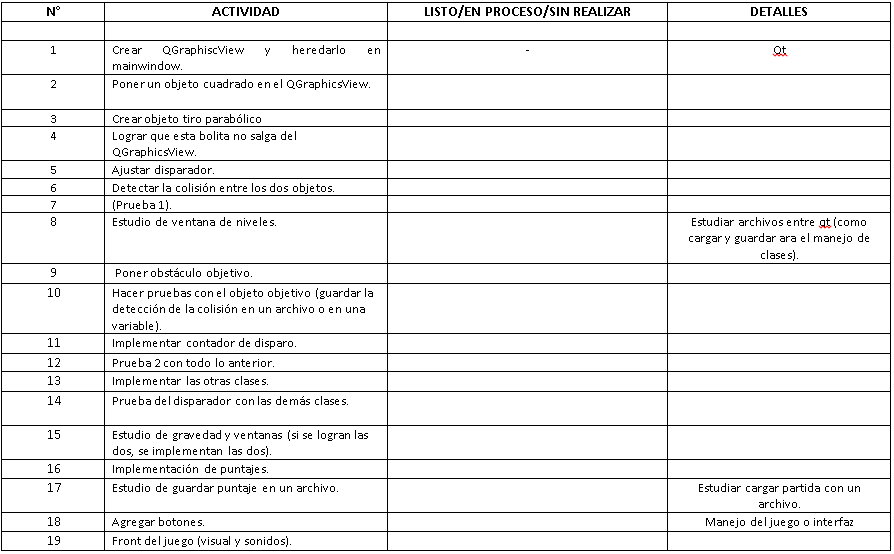
\includegraphics[width=1.1\textwidth]{Fechas1.PNG}
\caption{\label{fig1}Actividades}
\end{figure}
\\

\begin{figure}[h!]
\centering
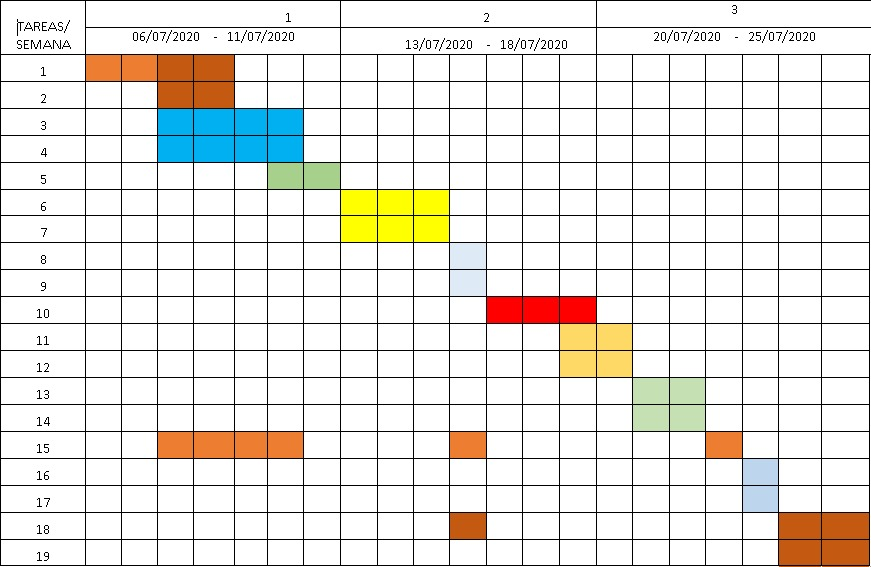
\includegraphics[width=1.1\textwidth]{prueba.png}
\caption{\label{fig1}Semana a semana}
\end{figure}
\\

\end{document}
